$y=\frac{1}{1+x^2}$, $y=0$, $x=\pm1$

\nopagebreak
\begin{align*}
A &= \int_{-1}^{1} \frac{dx}{1+x^2} \\
&= [\arctan x]_{-1}^{1} \\
&= \arctan(1) - \arctan(-1) \\
&= \frac{\pi}{4} - (-\frac{\pi}{4}) = \frac{\pi}{2}
\end{align*}

\[
\boxed{\displaystyle \frac{\pi}{2}}
\]

\begin{center}
    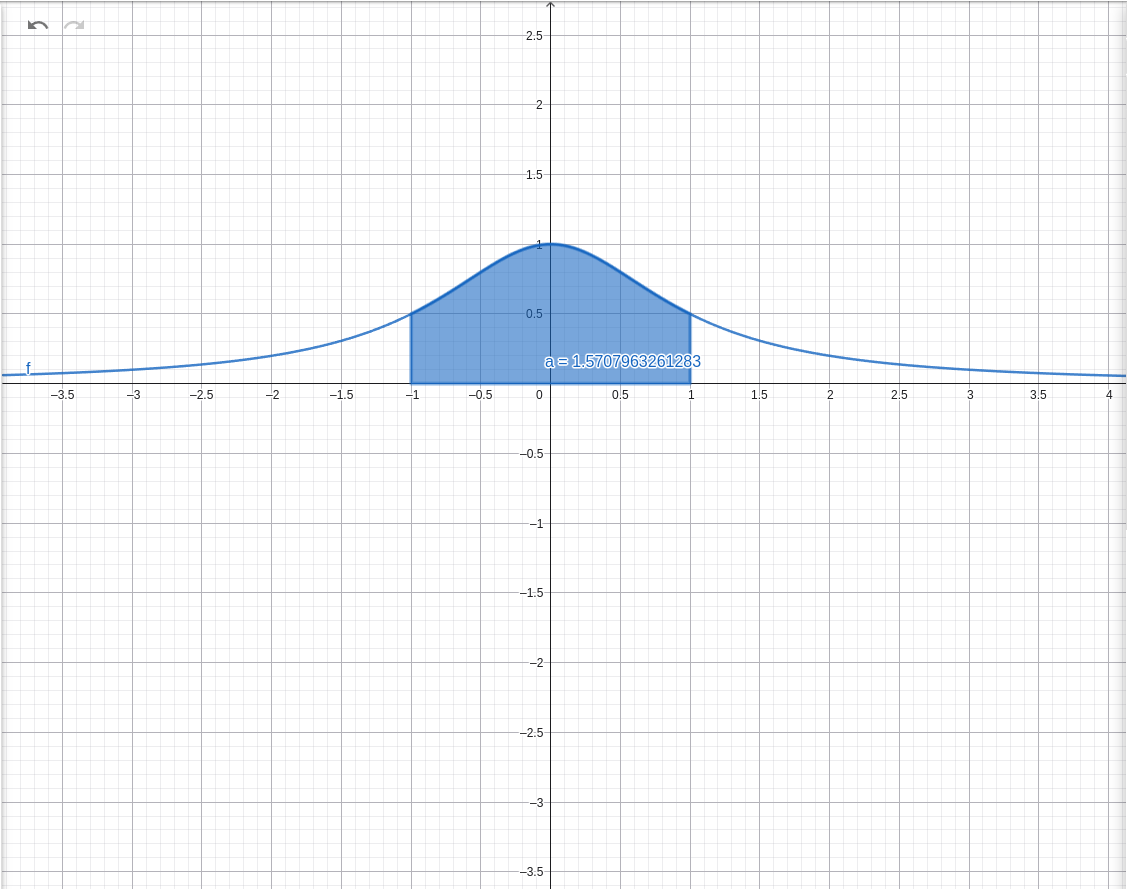
\includegraphics[width=0.5\textwidth]{Graficas/ejer24.png}
\end{center}
